\InputIfFileExists{../data/global.tex}\relax\relax

\iffull
\title{Von Erben, Scherben und dem Schnittstelle-werden}
\subtitle{The final Tut}
\date{KW 29}
\addbibresource{references.bib}
\fi
\SetTutoriumNumber{11}

\iffull\begin{document}
\titleframe

\TopicOverview{5}
\fi

\iffull{\SummaryFrame
\begin{frame}[c]{Kurzwiederholung}
\vspace*{1em}
\begin{center}
    \onslide<2->{Diesmal am Ende, als Zusammenfassung!}
\end{center}
\end{frame}
}\fi

% \SetNextSectionText[.6\linewidth]{TODO}
\section{Präsenzaufgabe}
{
\begin{frame}[fragile,c]{Präsenzaufgabe}
\begin{aufgabe}{Dir streichen wir das Erbe!}
    \only<2-3|handout:0>{Gegeben sei die folgende abstrakte Klasse RegularPolygon, welche ein Polygon mit gleichen Seitenlängen bzw. Innenwinkeln repräsentieren soll:}
\lstfs{9}%
\begin{minted}{java}
/*\onslide<3->*/public abstract class RegularPolygon {
/*\onslide<3->*/    protected final int numSides;
/*\onslide<3->*/    protected final double sideLength;
/*\onslide<3->*/    public RegularPolygon(int numSides, double sideLength) {
/*\onslide<3->*/        numSides = numSides;
/*\onslide<3->*/        sideLength = sideLength;
/*\onslide<3->*/    }
/*\onslide<3->*/    public int getNumSides() { return numSides; }
/*\onslide<3->*/    public double getCircumference() { return numSides * sideLength; }
/*\onslide<3->*/    public abstract double getArea();
/*\onslide<3->*/}
\end{minted}
\end{aufgabe}
\end{frame}
}

\SetNextSectionText{Dynamische Datenstrukturen II\\Abgabe: \DTMDate{2022-07-18}}
\section{Übungsblatt 11}
\subsection{Aufgabe 1}
{\taskenum
\begin{frame}[c]{Aufgabe 1: TODO}
    \taskblock<2->

    \endtaskblock
\end{frame}
}

\iffull
\SetNextSectionText{Fortgeschrittene OOP\\Abgabe: \T{null}}
\section[Aussicht: Übungsblatt \T{Integer.MAX\_VALUE}]{Aussicht: Übungsblatt \textbf{\T{Integer.MAX\_VALUE}}}
\subsection{Aufgabe 1}
\begin{frame}{Aufgabe 1: TODO}

\end{frame}
\fi

% \SetNextSectionText[.55\linewidth]{TODO}
\section{Abschließendes}

\iffull{\SummaryFrame
\def\sub#1#2{\node[font=\footnotesize\sffamily,scale=.715,align=center,gray,below=-2.65mm] at(#1.south) {\strut#2\strut};}
\setbeamerfont{description item}{series=\mdseries,shape=\itshape}
\begin{frame}[c]{Algorithmen}
\begin{tikzpicture}[@O]
    \node[below left,yshift=-1.4cm] at(current page.north east) {\LoadOverview{1}{}{}};
\end{tikzpicture}%
\begin{itemize}[<+(1)->]
   \itemsep14pt
   \item Totale Korrektheit \begin{description}[Partielle Korrektheit: ]
      \item[Terminiertheit:] \strut\onslide<+(1)->{Endliche Schritte für jede Eingabe}
      \item[Partielle Korrektheit:] \strut\onslide<+(1)->{Wenn terminiert, dann korrekt}
   \end{description}
   \item Weitere Eigenschaften \begin{description}[Determiniertheit: ]
      \item[Determiniertheit:] \strut\onslide<+(1)->{Gleiche Eingabe~\(\to\) Gleiche Ausgabe\infoblock{Einer determinierten Person ist egal, \textit{wie} sie ihr Ziel erreicht.}}
      \item[Determinismus:] \strut\onslide<+(1)->{Gleiche Eingabe~\(\to\) Gleiche Zustandsfolge}
   \end{description}
\end{itemize}\vfill
\centerline{%
\begin{tikzpicture}
    \onslide<+(1)->{\node (0) at(0,0) {\strut Spezifikation};
    \sub0{Begriffe mit\\Problemrelevanz}}
    \foreach[count=\i,remember =\i as \li (initially 0)] \a/\t in {Abstraktion/{Gegeben \& Gesucht},{\makebox[14mm]{\only<17->{\sbseries}Entwurf}}/{Algorithmus},Verifikation/{Termination \&\\partielle Korrektheit},Aufwandsanalyse/{Laufzeitverhalten}} {
        \onslide<+(1)->{\node[right=.5mm] (k\i) at(\li.east) {\strut\faAngleRight};
        \node[right=.5mm] (\i) at (k\i.east) {\strut\a};
        \sub\i{\t}}
    }
\end{tikzpicture}}
\end{frame}

\def\mto{\ensuremath{\to}}
\def\dt#1{{\textcolor{paletteA!58!white}{\sbseries\strut#1}}}
\begin{frame}[c]{Konstrukte}
\begin{tikzpicture}[@O]
    \node[below left,yshift=-1.4cm] at(current page.north east) {\LoadOverview{2}{}{}};
\end{tikzpicture}%
\begin{itemize}[<+(1)->]
   \itemsep15pt
   \item \textit{Implizit}:\quad\pause \dt{byte}~\mto~\dt{short}~\mto~\dt{int}~\mto~\dt{long}~\mto~\dt{float}~\mto~\dt{double}\\
   Zahlen von klein zu groß, sowie: \dt{char}~\mto~\dt{int}
   \item \textit{Präzedenzregeln}:\pause\\
   Post vor Prä, sonst wie Arithmetik \& Logik
   \item \textit{Default-Werte}:\quad\pause Zahlen und Zeichen \bjava{0}, Boolean \bjava{false}, Rest \bjava{null}\pause\\
   Nur bei: Arrays, Instanz- und Klassenvariablen (\link{https://docs.oracle.com/javase/specs/jls/se17/html/jls-4.html\#jls-4.12.5}{JLS17~4.12.5})
   \item \textit{Überschatten}:\pause\\
   Lokaler Bezeichner überdeckt Gültigkeit des globalen
\end{itemize}
\end{frame}

\def\mto{\ensuremath{\to}}
\begin{frame}[c]{Arrays \& Iteration}
\begin{tikzpicture}[@O]
    \node[below left,yshift=-1.4cm] at(current page.north east) {\LoadOverview{3}{}{}};
\end{tikzpicture}%
\begin{itemize}[<+(1)->]
   \itemsep15pt
   \item Arrays sind komplexe Datentypen
   \item Mehrdimensionale Arrays sind eindimensionale Arrays von\\seindimensionalen Arrays von\ldots
   \item Die drei Schleifenarten sind gleich mächtig \begin{itemize}
      \item Maximum bekannt: \bjava{for}
      \item Mindestens ein mal: \bjava{do}-\bjava{while}
      \item Sonst: \bjava{while}
   \end{itemize}
\end{itemize}
\end{frame}

\begin{frame}[c]{Unterprogramme}
\begin{tikzpicture}[@O]
    \node[below left,yshift=-1.4cm] at(current page.north east) {\LoadOverview{4}{}{}};
\end{tikzpicture}%
\begin{itemize}[<+(1)->]
   \itemsep15pt
   \item \textit{Überladung:}\quad\pause Gleicher Name, andere Signatur \begin{itemize}
      \item \textit{Signatur:} \pause Name \& Parametertypliste
      \item Müssen zudem in selber Klasse sein (später: Vererbung)
   \end{itemize}
   \item Beim Aufruf macht Java call-by-value: \begin{itemize}
      \item Alle Parameter werden kopiert (Stack)
   \end{itemize}
   \item \bjava{void} gibt als Keyword an, dass die Methode keinen Rückgabetyp hat
\end{itemize}
\end{frame}

\begin{frame}[c]{Objektorientierte Progammierung}
\begin{tikzpicture}[@O]
    \node[below left,yshift=-1.4cm] at(current page.north east) {\LoadOverview{5}{}{}};
\end{tikzpicture}%
\begin{itemize}[<+(1)->]
   \itemsep10pt
   \item Eine Klasse definiert die Blaupause für Objekte \begin{itemize}
      \item Attribute definieren den Zustand
      \item Methoden definieren den Verhalten
      \item Statische Elemente sind nicht Teil der Blaupause \info{sie gehören der Klasse!}
   \end{itemize}
   \item Der Konstruktor baut den initialen Zustand \begin{itemize}
      \item \textit{Instanziierung}: \pause Erzeugen eines neuen Objektes
      \item Wenn keiner: \pause erzeugt Java den leeren Standardkonstruktor
      \item \bjava{this} erlaubt Aufruf von überladenen Konstruktoren
   \end{itemize}
   \item Klassen, Methoden,~\ldots:\quad \textit{Sichtbarkeit} (\bjava{public},~\ldots)
   \item \textit{Gültigkeit}sbereich:\quad Wo die Variablen \say{deklariert sind} (Überschatten,~\ldots)
\end{itemize}
\end{frame}

\begin{frame}[fragile,c]{Rekursion}
\lstfs{8}
\begin{tikzpicture}[@O]
    \node[below left,yshift=-1.4cm] at(current page.north east) {\LoadOverview{7}{}{}};
\end{tikzpicture}%
\begin{itemize}[<+(1)->]
\itemsep8pt
    \item<2-> Methoden, die sich direkt oder indirekt selbst aufrufen sind rekursiv.
    \begin{itemize}
        \itemsep1.5pt
        \item<3-> Ruft sich eine Methode maximal einmal selbst auf, ist sie \textit{linear rekursiv}.
\begin{columns}[c]
\column{.35\linewidth}
    \onslide<4->{\(\displaystyle f(x) = \begin{cases}
        1 & \text{ if } x < 2 \\
        f(x - 1) \cdot x & \text{ otherwise }
    \end{cases}\)}
\column{.45\linewidth}
\begin{minted}{java}
/*\onslide<5->*/public int f(int x) {
/*\onslide<6->*/    if(x < 2) return 1;
/*\onslide<7->*/    else return f(x - 1) * x;
/*\onslide<5->*/}/*\onslide<1->*/
\end{minted}
\end{columns}
        \item<8-> \textit{Kopfrekursiv}, wenn dieser Aufruf das erste Statement ist \info{alles passiert im Aufstieg}
        \item<9-> \textit{Endrekursiv}, wenn dieser Aufruf das letzte Statement ist \info{alles passiert im Abstieg}\vspace*{-\medskipamount}
\begin{columns}[c]
\column{.35\linewidth}
\begin{minted}{java}
/*\onslide<10->*//*\CodeMarker{\textbf{Head}-Recursive}*/
/*\onslide<10->*/public int f(int x) {
/*\onslide<10->*/    if(x < 2) return 1;
/*\onslide<10->*/    else return f(x - 1) * x;
/*\onslide<10->*/}/*\onslide<1->*/
\end{minted}
\column{.45\linewidth}
\begin{minted}{java}
/*\onslide<11->*//*\CodeMarker{\textbf{Tail}-Recursive, call as f(x, 1)}*/
/*\onslide<11->*/public static int f(int x, int acc) {
/*\onslide<11->*/    if(x < 2) return acc;
/*\onslide<11->*/    else return f(x - 1, acc * x);
/*\onslide<11->*/}/*\onslide<1->*/
\end{minted}
\end{columns}\vspace*{-\smallskipamount}
        \item<12-> Ruft sie sich auch mehrfach pro Rekursionsfall auf, ist sie \textit{verzweigt rekursiv}.
    \end{itemize}
\end{itemize}
\end{frame}

\let\oldO\O
\def\O(#1){#1}
\begin{frame}[fragile,c]{Suchen und Sortieren}
\lstfs{8}
\begin{tikzpicture}[@O]
    \node[below left,yshift=-1.4cm] at(current page.north east) {\LoadOverview{9}{}{}};
\end{tikzpicture}%
\onslide<2->{%
\def\arraystretch{1.225}%
\begin{tabular}{ll*2{l}>{\footnotesize}{l}}
              & & \multicolumn{2}{c}{Laufzeit \info{\(\oldO(\ldots)\)}}  & \vspace*{-\smallskipamount}\\
    \cmidrule{3-4}
    \onslide<2->{\rotatebox{90}{\rlap{\footnotesize Stabil?}}} & & \onslide<2->{best} & \onslide<2->{worst} & \onslide<2->{\normalsize Ansatz} \medskip\\
    \onslide<4->{\(\checkmark\)} & \onslide<3->{\tikzmarknode{itstart}{Bubble}}      & \onslide<3->{\(\O(n^2)\)\textcolor{gray}{, \(\O(n)\)}}       & \onslide<3->{\(\O(n^2)\)} & \onslide<4->{Vertausche benachbarte El., solange unsortiert.} \\
    \onslide<6->{\(\checkmark\)} & \onslide<5->{Insertion} & \onslide<5->{\(\O(n)\)}             & \onslide<5->{\(\O(n^2)\)}      & \onslide<6->{Sortiere 1. unsortiertes El. in sortierten Teil ein.}\\
    & \onslide<7->{\tikzmarknode{itend}{Selection}} & \onslide<7->{\(\O(n^2)\)}    & \onslide<7->{\(\O(n^2)\)}      & \onslide<8->{Kleinstes unsortiertes El. an Ende des sortierten Teils.} \medskip\\
    % Quick-, merge und Heapsort können auch O(n)
    \onslide<10->{\(\checkmark\)} & \onslide<9->{\tikzmarknode{rekstart}{Merge}}    & \onslide<9->{\(\O(n \log n)\)} & \onslide<9->{\(\O(n \log n)\)}  & \onslide<10->{Aufteilen bis einel., wiederholtes mergen sortierter Teillisten.}\\
    & \onslide<11->{Quick}                             & \onslide<11->{\(\O(n \log n)\)} & \onslide<11->{\(\O(n^2)\)}    & \onslide<12->{Pivot $\to$ Ende, \(\ell\) solang \(<\), \(r\) solang \(\geq\). Treffen \(\to\) tausche Pivot.}\\
    & \onslide<13->{\tikzmarknode{rekend}{Heap}}       & \onslide<13->{\(\O(n \log n)\)} & \onslide<13->{\(\O(n\log n)\)} & \onslide<14->{Baue Heap, entferne wiederholt Wurzel, heapify.}
\end{tabular}\bigskip\par
\only<0|handout:1>{\scriptsize\textit{Dies folgt den Implementationen der Vorlesung. Bereits leichte Modifikationen (wie: prüfe zuerst ob die Liste bereits sortiert ist) können die Daten verändern (beispielsweise einen best-case von \(\O(n)\) im Falle von Bubblesort).}\par}}
\end{frame}

\def\treenode[#1](#2)#3#4{\node[draw,rounded corners=2pt,minimum width=.75cm,minimum height=7mm,align=center,#1] (#3) at (#2) {#4\\[-.35mm]};\draw([yshift=-.5mm]#3.east) -- ([yshift=-.5mm]#3.west) coordinate[pos=.5] (@); \draw(@) -- (#3.south);}
\begin{frame}[fragile,t]{Dynamische Datenstrukturen}
\lstfs{7}%
\begin{tikzpicture}[@O]
    \node[below left,yshift=-1.4cm] at(current page.north east) {\LoadOverview{6}{}{}};
\end{tikzpicture}%
\begin{description}[Einfach verketteter Binärbaum:]
    \itemsep25pt
    \item<2->[Einfach verkettete Liste:] ~\onslide<3->{\tikzset{W/.style={draw, rounded corners=2pt},K/.style={W, rectangle split, rectangle split parts=2,rectangle split horizontal}}\scalebox{.8}{\begin{tikzpicture}[align-half-base]
    \node[K] (a) at (0,0) {4\nodepart{two}};
    \node[K,right=2mm] (b) at (a.east) {5\nodepart{two}};
    \node[K,right=2mm] (c) at (b.east) {1\nodepart{two}};
    \node[K,right=2mm] (d) at (c.east) {3\nodepart{two}};
    \node[W,right=2mm] (e) at (d.east) {\phantom{2}};
    \pgfinterruptboundingbox
    \node[below=-.33mm,T] at (a.south) {head};
    \node[below=-.33mm,T] at (d.south) {(tail)};
    \endpgfinterruptboundingbox
    \draw[shorten <= .4mm,shorten >= .4mm,] (e.south west) -- (e.north east);
    \draw[Circle-Kite] ([xshift=-1.65ex]a.east) -- (b.west);
    \draw[Circle-Kite] ([xshift=-1.65ex]b.east) -- (c.west);
    \draw[Circle-Kite] ([xshift=-1.65ex]c.east) -- (d.west);
    \draw[Circle-Kite] ([xshift=-1.65ex]d.east) -- (e.west);
\end{tikzpicture}}}
% this is horrible, but i have no time
    \item<4->[Doppelt verkettete Liste:] ~\onslide<5->{\tikzset{W/.style={draw, rounded corners=2pt},K/.style={W, rectangle split, rectangle split parts=3,rectangle split horizontal}}\scalebox{.8}{\begin{tikzpicture}[align-half-base]
    \node[K] (a) at (0,0) {\nodepart{two}4\nodepart{three}};
    \node[W,left=2mm] (f) at (a.west) {\phantom{2}};
    \node[K,right=2mm] (b) at (a.east) {\nodepart{two}5\nodepart{three}};
    \node[K,right=2mm] (c) at (b.east) {\nodepart{two}1\nodepart{three}};
    \node[K,right=2mm] (d) at (c.east) {\nodepart{two}3\nodepart{three}};
    \node[W,right=2mm] (e) at (d.east) {\phantom{2}};
    \pgfinterruptboundingbox
    \node[below=-.33mm,T] at (a.south) {head};
    \node[below=-.33mm,T] at (d.south) {tail};
    \endpgfinterruptboundingbox
    \draw[shorten <= .4mm,shorten >= .4mm,] (e.south west) -- (e.north east);
    \draw[shorten <= .4mm,shorten >= .4mm,] (f.south west) -- (f.north east);
    \draw[Circle-Kite] ([yshift=1mm,xshift=-1.65ex]a.east) -- ([yshift=1mm]b.west);
    \draw[Circle-Kite] ([yshift=-1mm,xshift=1.65ex]b.west) -- ([yshift=-1mm]a.east);
    \draw[Circle-Kite] ([yshift=1mm,xshift=-1.65ex]b.east) -- ([yshift=1mm]c.west);
    \draw[Circle-Kite] ([yshift=-1mm,xshift=1.65ex]c.west) -- ([yshift=-1mm]b.east);
    \draw[Circle-Kite] ([yshift=1mm,xshift=-1.65ex]c.east) -- ([yshift=1mm]d.west);
    \draw[Circle-Kite] ([yshift=-1mm,xshift=1.65ex]d.west) -- ([yshift=-1mm]c.east);
    \draw[Circle-Kite] ([xshift=-1.65ex]d.east) -- (e.west);
    \draw[Circle-Kite] ([xshift=1.65ex]a.west) -- (f.east);
\end{tikzpicture}}}
    \item<6->[Einfach verketteter Binärbaum:] ~\tikzset{W/.style={draw, rounded corners=2pt}}%
    \onslide<7->{\smash{\raisebox{-.5\height}{\rotatebox{90}{\scalebox{.6}{\begin{tikzpicture}[align-half-base]
    \treenode[](0,0)a{\rotatebox{-90}{4}};
    \treenode[yshift=-2mm,below left=2mm](a.south)b{\rotatebox{-90}{5}};
    \treenode[yshift=-2mm,below right=2mm](a.south)c{\rotatebox{-90}{1}};
    \treenode[yshift=-2mm,below left=2mm](b.south)d{\rotatebox{-90}{3}};
    \node[W,yshift=-2mm,xshift=1mm,below left=2mm] (e) at (d.south) {\phantom{2}};
    \node[W,yshift=-2mm,xshift=-1mm,below right=2mm] (f) at (d.south) {\phantom{2}};
    \node[W,yshift=-2mm,xshift=1mm,below left=2mm] (g) at (c.south) {\phantom{2}};
    \node[W,yshift=-2mm,xshift=-1mm,below right=2mm] (h) at (c.south) {\phantom{2}};
    \node[W,yshift=-2mm,xshift=-1mm,below right=2mm] (i) at (b.south) {\phantom{2}};
    \foreach \a in {e,...,i} {
        \draw[shorten <= .4mm,shorten >= .4mm,] (\a.south east) -- (\a.north west);
    }
    \foreach \fr/\tol/\tor in {a/b/c,b/d/i,c/g/h,d/e/f} {
        \draw[Circle-Kite] ([xshift=-.75cm/4,yshift=2mm]\fr.south) -- (\tol.north);
        \draw[Circle-Kite] ([xshift=.75cm/4,yshift=2mm]\fr.south) -- (\tor.north);
    }
    \node[left,T] at (a.west) {\rotatebox{-90}{root}};
\end{tikzpicture}}}}}}
% TODO: example code traversal
% TODO: example code list append
\begin{tikzpicture}[@O]
\begin{onlyenv}<8->
\node[above right,xshift=5mm,yshift=\btdmfootheight+.25cm,text width=5cm] at(current page.south west) {%
\begin{minted}{java}
void inorder(Node n)  {
    if (n == null) return;
    inorder(n.left);
    System.out.println(n.value);
    inorder(n.right);
}
\end{minted}
};
\end{onlyenv}
\begin{onlyenv}<9->
\node[above left,xshift=-6.5mm,yshift=\btdmfootheight+1.5cm,text width=6.5cm] at(current page.south east) {%
\begin{minted}[morekeywords={[3]{Elem}}]{java}
private class Elem {
  public final int value;
  public Elem prev, next;
  public Elem(int v, Elem p, Elem n) {
    value = v; prev = p; next = n;
  }
}
\end{minted}
};
\end{onlyenv}
\begin{onlyenv}<10->
    \node[above left,xshift=-.5mm,yshift=\btdmfootheight-.25cm,text width=6cm] at(current page.south east) {%
    \begin{minted}[morekeywords={[3]{Elem}}]{java}
Elem head, tail;
public void addFront(int value) {
    Elem elem = new Elem(value, null, head);
    if(head == null) tail = elem;
    else head.prev = elem;
    head = elem;
}
\end{minted}
};
\end{onlyenv}
\end{tikzpicture}
\end{description}
\end{frame}
}\fi

\outro{\vskip9mm\centering \onslide<2->{\scalebox{1.75}{

}}}

\iffull\end{document}\fi
